\section{\texorpdfstring{$\infty$}--category via Simplicial Sets}

With the definitions of horns and simplices settled, we are now ready to present one defintion of small $\infty$-categories via simplicial sets.

\subsection{Weak Kan Extension Condition}

\begin{definition}[$\infty$-category]\label{def:infinity-cat}
	An $\infty$-category, $\mathcal{D}$ is a simplicial set that satisfies the inner horn-filling conditions.

	Specifically, for each $n \geq 2$ and $0 < i < n$, any map of from the $i$th horn $f: \L^n_i \to \mathcal{D}$ can be extended to a map $\overline{f}: \Delta^n \to \mathcal{D}$ such that the following diagram commutes:

$$
\begin{tikzpicture}[>=Stealth]
  % Nodes
	\node (A) {$\L^n_i$};
	\node[right=of A] (B) {$\mathcal{D}$};
	\node[below=of A] (C) {$\Delta^n$};

  % Arrows (legs of the right triangle)
	\draw[->] (A) -- node[above] {$f$} (B);
	\draw[->, dotted] (C) -- node[below right] {$\exists \tilde{f}$} (B);

  \draw[right hook->] (A) -- node[below left] {} (C);
\end{tikzpicture}
$$

The maps between simplicial sets are natural transformations in $[\D\op, \S]$.
There is no requirement for uniqueness of the extension.

This condition is also known as the \emph{weak Kan extension condition}, and $\infty$-category is also called \emph{weak Kan complex} \cite{boardman2006homotopy}.
\end{definition}

\begin{remark}
	The reason for calling it \textit{weak} Kan complex is because we have a different condition for \emph{Kan complex}, which requires filling all horns, including the outer horns.
\end{remark}


In the language of model categories, $\infty$-categories are precisely the fibrant objects in the Joyal model structure on $\sS$ \cite{joyal}.

In this definition, the objects of the $\infty$-category $\mathcal{D}$ are given by the $0$-simplices $\mathcal{D}_0$, the morphisms between two objects $x, y \in \mathcal{D}_0$ are given by the $1$-simplices $f \in \mathcal{D}_1$ such that $d_1(f) = x$ and $d_0(f) = y$. 
Higher objects are given by higher simplices in a similar manner.

The inner horn-filling condition precisely encodes the composition of morphisms and higher homotopies between them.
Figure \ref{fig:infinity-cat-composition} explains the composition of $1$-simplices.

A map of simplicial set $\L^2_1 \rightarrow \mathcal{D}$ consists of two $1$-simplices $f, g \in \mathcal{D}_1$ such that $d_0(f) = d_1(g)$, as shown on the left figure \ref{fig:infinity-cat-composition}.
An extension of this map to $\Delta^2 \to \mathcal{D}$ gives a $2$-simplex in $\sigma$ that fills the horn, with the condition that $d_2(\sigma) = f$ and $d_0(\sigma) = g$, as shown on the right of the following diagram.
Therefore, we may define the composition of $f$ and $g$ via the face map $g \circ f = d_1(\sigma)$.

Note the the inner horn-filling need not be unique, so the composition may not be unique either.
We will show later that the composition is unique up to homotopy.

% Demonstration of composition
\begin{figure}
	\centering 
\begin{tikzpicture}[every node/.style={font=\small}, line cap=round, scale=0.8]
  % coordinates
  \coordinate (L) at (0,0);      % left vertex
  \coordinate (R) at (3,0);      % right vertex
  \coordinate (T) at (1.5,2);    % top vertex

  % vertices as filled circles
  \node[draw,fill,inner sep=1.8pt, circle] (vL) at (L) {};
  \node[draw,fill,inner sep=1.8pt, circle] (vR) at (R) {};
  \node[draw,fill,inner sep=1.8pt, circle] (vT) at (T) {};

  % edges with labels
  \draw[thick] (vL) -- node[midway, left] {$f$} (vT);
  \draw[thick] (vT) -- node[midway, right] {$g$} (vR);

  % labels for vertices
  \node[below left=2pt of vL]  {$d_1(f)$};
  \node[below right=2pt of vR] {$d_0(g)$};
  \node[above=2pt of vT]       {$d_0(f)=d_1(g)$};

\end{tikzpicture}
\qquad \qquad
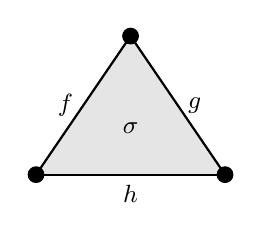
\begin{tikzpicture}[line cap=round, font=\small, scale=0.8]

  % coordinates
  \coordinate (L) at (0,0);
  \coordinate (R) at (3,0);
  \coordinate (T) at (1.5,2.2);
  % \node at ($(L)+(R)+(T)/3$) {$\sigma$};

  % shaded triangle
  \fill[gray!20] (L) -- (R) -- (T) -- cycle;

  % edges
  \draw[thick] (L) -- node[midway, below] {$h$} (R);
  \draw[thick] (L) -- node[midway, left] {$f$} (T);
  \draw[thick] (T) -- node[midway, right] {$g$} (R);

  % vertices
  \foreach \p in {L,R,T}
    \node[draw, fill, circle, inner sep=2pt] at (\p) {};

	\node at (barycentric cs:L=1,R=1,T=1) {$\sigma$};
\end{tikzpicture}
\caption{Composition of 1-simplices via inner horn-filling condition}
\label{fig:infinity-cat-composition}
\end{figure}


Let us now give some examples of $\infty$-categories.

\begin{example}
	$\Delta^0$ gives the trivial $\infty$-category with one object and one morphism.
\end{example}

\begin{example}
	In general $\Delta^k$ is a an $\infty$-category for all positive integer $k$.
	The reason is the following.

	Since we only need to fill the inner horns, we only need to consider simplicial maps from $\L^n_i$ to $\Delta^k$ for $n \geq 2$.
	Take $\L^2_1$ for example, we want to fill the horn by finding an extension of the map $f: \L^2_1 \to \Delta^k$ to $g: \Delta^2 \to \Delta^k$.

	We may have an intuitive arguments through the figure \ref{fig:infinity-cat-composition}. 
	Since $\L^2_1$ contains all the vertices of $\Delta^2$, the map $f$ sends the three vertices of $\Delta^2$ to three vertices in $\Delta^k$, which forms a $2$-simplex in $\Delta^k$.
	Therefore, we can just identify $\Delta^2$ as the image $f(\Delta^2)$ in $\Delta^k$.
	In fact, we can see this is the unique extension, and $\Delta^k$ is a actually a Kan complex.


	If the above argument is not convincing enough, let us wade through the commutative diagrams.
	Consider the following commutative diagram.
$$
\begin{tikzpicture}[->, >=Stealth]
  % Nodes
	\node (A) {$\Delta^2[1]$};
	\node[right=of A] (B) {$\Delta^2[0]$};
	\node[below=of B] (C) {$\Delta^k[0]$};
	\node[below=of A] (D) {$\Delta^k[1]$};

  % Arrows (legs of the right triangle)
  \draw (A) -- node[above] {$d_1$} (B);
  \draw (A) -- node[right] {$g_1$} (D);
  \draw (B) -- node[right] {$g_0$} (C);
  \draw (D) -- node[below] {$d_1$} (C);

\end{tikzpicture}
$$

There is only one element in $\Delta^2[1]$ that is not contained in $\L^2_1[1]$, namely this element is $\alpha: [1] \rightarrow [2]$ that send $0$ to $0$ and $1$ to $2$.
Let us take this element through the above commutative diagram.

Note that $d_1 \alpha \in \Delta^2[0]$ is the map that sends $0$ to $0$, which is contained in $\L^2_1[0]$.
By horn-filling condition must equal to $d_1 f_0(\alpha)$
Similarly, $d_0 \alpha = d_0 f_0(\alpha)$.
Notice that in $\Delta^k$ there is a unique 1-simplex $\eta$ such that $d_1 \eta = d_1 f_0(\alpha)$ and $d_0 \eta = d_0 f_0(\alpha)$, and we shall define $g_1(\alpha) = \eta$.

How the natural transformation $g$ acts on the rest of simplices can be defined similarly.
\end{example}


\subsection{Nerves of Categories}

Our first examples of $\infty$-category are the nerves of ordinary categories.

\begin{definition}[Nerves]
	Let $\mathcal{C}$ be an ordinary category.
	Regard $[n]$ as an ordinary category where the objects are elements in $[n]$ and there is a unique morphism from $i$ to $j$ if and only if $i \leq j$.
	The \emph{nerve} of $\C$, denoted as $N(\C)$, is the simplicial set defined as
	\begin{enumerate}
		\item The $n$-simplices are the set of functors from $[n]$ to $\C$, i.e.,
			\begin{equation*}
				N(\C)_n := N(\mathcal{C})([n]) = \F_{\text{Cat}}([n], \mathcal{C}),
			\end{equation*}
		\item The structure maps are induced by the pullbacks along morphisms in $\D$.
			That is for $f \in \H_{\D}([m], [n])$ and $G \in N(\C)([n])$, $N(\C)(f): N(\C)_n \rightarrow N(\C)_m$
			\begin{equation*}
				N(\C)(f) (G) = G \circ f
			\end{equation*}
	\end{enumerate}
\end{definition}

Recall the category $[n]$ is the category induced by the order in the set 
$$\{0 \leq 1 \leq 2 \leq 3 \leq \cdots \leq n\},$$
where a unique morphism exists from $i$ to $j$ if and only if $i \leq j$. 
This is indeed a category, as the identity morphisms of the element $i$ is represented by $i \leq i$, and any compositions of morphisms leads to a unique morphism due to the transitivity of the order relation.

A function from $[n]$ to $\C$ is, therefore, precisely $n+1$ objects in $\C$ with a chain of $n$ morphisms between them, as shown below.
\begin{equation}\label{Nerve-n-chain}
	X_0 \xrightarrow{f_1} X_1 \xrightarrow{f_2} X_2 \xrightarrow{f_3} X_3 \xrightarrow{f_{4}} \cdots \xrightarrow{f_n} X_{n}
\end{equation}
Specifically, $N(\C)_0$ is precisely the objects in $\C$, and $N(\C)_1$ is the collection of morphisms in $\C$.

\begin{remark}\label{nerve-encodes-cat}
	Because $N(\C)_0$ is the objects in $\C$, and $N(\C)_1$ is the morphisms in $\C$, the nerve $N(\C)$ encodes all the data of the ordinary category $\C$. 
\end{remark}

\begin{remark}\label{nerve-face-deg}
Basic chasing of diagrams shows that the face map, $d_i: N(\C)_{n} \rightarrow N(\C)_{n-1}$ sends $n$-chain in \ref{Nerve-n-chain} to $(n-1)$-chain in the following way:
\begin{enumerate}
	\item if $i = 0$, it removes the first object and the first morphism, i.e., \ref{Nerve-n-chain} is sent to
		\begin{equation}
			X_1 \xrightarrow{f_2} X_2 \xrightarrow{f_3} X_3 \xrightarrow{f_{4}} \cdots \xrightarrow{f_n} X_{n}
		\end{equation}
	\item if $0 < i < n$, it removes the $i$-th object and composes the $(i-1)$-th and $i$-th morphisms, i.e., \ref{Nerve-n-chain} is sent to
		\begin{equation}
			X_0 \xrightarrow{f_1} \cdots \xrightarrow{f_{i-1}} X_{i-1} \xrightarrow{f_{i+1} \circ f_i} X_{i+1} \xrightarrow{f_{i+2}} \cdots \xrightarrow{f_n} X_{n}
		\end{equation}
	\item if $i = n$, it removes the last object and the last morphism, i.e., \ref{Nerve-n-chain} is sent to
		\begin{equation}
			X_0 \xrightarrow{f_1} X_1 \xrightarrow{f_2} X_2 \xrightarrow{f_3} \cdots \xrightarrow{f_{n-1}} X_{n-1}
		\end{equation}
\end{enumerate}

Similarly, the degenerate map $s_i: N(\C)_n \to N(\C)_{n+1}$ sends the $n$-chain in \ref{Nerve-n-chain} to the $(n+1)$-chain
\begin{equation}
	X_0 \xrightarrow{f_1} \cdots \xrightarrow{f_{i}} X_{i} \xrightarrow{\text{id}_{X_i}} X_i \xrightarrow{f_{i+1}} \cdots \xrightarrow{f_n} X_{n}
\end{equation}
\end{remark}

The nerves by construction are simplicial sets. An important property is that they are also $\infty$-categories, as stated in the following theorem.

\begin{theorem}
	Let $\C$ be an ordinary category.
	Its nerve $N(\C)$ satisfies the inner horn-filling conditions; therefore is an $\infty$-category.
	Moreover, the extension $\overline{f}: \Delta^n \to N(\C)$ of the map $f: \L^n_i \to N(\C)$ is unique.
\end{theorem}

$$
\begin{tikzpicture}[>=Stealth]
  % Nodes
	\node (A) {$\L^n_i$};
	\node[right=of A] (B) {$\C$};
	\node[below=of A] (C) {$\Delta^n$};

  % Arrows (legs of the right triangle)
	\draw[->] (A) -- node[above] {$f$} (B);
	\draw[->, dotted] (C) -- node[below right] {$\exists ! \tilde{f}$} (B);

  \draw[right hook->] (A) -- node[below left] {} (C);
\end{tikzpicture}
$$

\begin{proof}
	Because inner horns are $\L^i_n$ such that $0 < i < n$, we only need to consider the cases for $n \geq 2$.

	Notice $\L^i_n$ has $n$ vertices (the set of vertices is $\L^i_n[0]$). Lable these vertices as $X_0, X_1, \cdots, X_n$.
	Given $f$, we want to find a natural transformations $\tilde{f}\in [\D\op, \S]$, that is, a class of maps $\alpha_{[n]}: \Delta^n \rightarrow N(\C)_n$.

	Notice $\alpha_{[0]}$, a set of $n$ vertices, is completely determined by $f$, so is any $\alpha_{[k]}$ for $k < n - 1$, as $\L^i_n$ only misses one $(n-1)$-simplex, which is the $i$th face, and the only $n$-simplex.
	Therefore, we have the $n$-chain of objects and morphisms in $\C$:
	\begin{equation*}
		X_0 \xrightarrow{f_1} X_1 \xrightarrow{f_2} X_2 \xrightarrow{f_3} X_3 \xrightarrow{f_{4}} \cdots \xrightarrow{f_n} X_{n}
	\end{equation*}
	Where $X_j = \alpha_{[0]}(j)$ and $f_j$ is the morphism from $X_{j-1}$ to $X_j$ induced by $\alpha_{[1]}$. 
	The existence of $f_i$ is clear for $n \geq 3$. 
	For $n = 2$, the only inner horn is $\L^2_1$, which contains the morphisms from $X_0$ to $X_1$ and from $X_1$ to $X_2$, so $f_1$ and $f_2$ are also well-defined.

	This is precisely $\alpha_{[n]}[n]$ we are looking for.
	And the missing $i$-th face is given by the face map $d_i$ applied to this $n$-chain.

\end{proof}

As a result, nerves of ordinary categories provide a large class of examples of $\infty$-categories.
